\documentclass[border=12pt]{standalone}
\def\pgfsysdriver{pgfsys-dvisvgm.def}
\usepackage[dvisvgm]{xcolor}
\usepackage{xeCJK}
\setCJKmainfont{HaranoAjiGothic-Regular.otf}[BoldFont=HaranoAjiGothic-Bold.otf]
\setCJKsansfont{HaranoAjiGothic-Regular.otf}[BoldFont=HaranoAjiGothic-Bold.otf]
\usepackage{amsmath,amssymb,tikz,lmodern}
\usetikzlibrary{arrows.meta,positioning,calc,fit,backgrounds}
\renewcommand{\familydefault}{\sfdefault}
\definecolor{ink}{HTML}{25322F}
\definecolor{green}{HTML}{246657}
\definecolor{tint}{HTML}{EEF4F0}
\definecolor{soft}{HTML}{C6D2CC}
\definecolor{muted}{HTML}{52615B}
\newif\ifJapanese
\newcommand{\Tx}[2]{\ifJapanese #1\else #2\fi}
\newcommand{\Eff}{\overline{\operatorname{Eff}}}
\newcommand{\heading}[3]{{\color{green}\bfseries #1\quad\Tx{#2}{#3}}\\[5pt]}
% A white rectangle makes the complete citation label clickable, including spaces.
\newcommand{\refurl}[2]{\special{dvisvgm:raw <a xlink:href="#1" target="_blank" rel="noopener noreferrer">}{\setlength{\fboxsep}{0pt}\colorbox{white}{\color{green}\underline{\strut #2}}}\special{dvisvgm:raw </a>}}
\newcommand{\refedge}[3]{\refurl{\csname source#1\endcsname\string##page=#2}{#3}}
\newcommand{\SF}[2]{\refedge{sf}{#1}{#2}}
% GitHub's file preview does not support PDF page fragments.
\newcommand{\LA}[2]{\refurl{\sourcela}{#2}}
\newcommand{\Sch}[2]{\refedge{sch}{#1}{#2}}
\newcommand{\PS}[2]{\refedge{ps}{#1}{#2}}
\tikzset{
 card/.style={draw=soft,fill=white,rounded corners=2pt,align=left,text=ink,font=\fontsize{10.5}{14}\selectfont,inner xsep=12pt,inner ysep=10pt,text width=14.4cm},
 half/.style={card,text width=6.45cm,minimum height=2.05cm},
 result/.style={card,draw=green,fill=tint,line width=.9pt},
 reason/.style={align=left,text=muted,font=\fontsize{9}{12}\selectfont,inner sep=0pt,text width=12.7cm},
 branchreason/.style={reason,text width=5.95cm},
 edge/.style={-{Stealth[length=2.4mm]},draw=green,line width=1pt},
 wire/.style={draw=green,line width=1pt},
}
% Keep the arrow in a dedicated left gutter; explanations never cover it.
\newcommand{\flow}[3]{
 \coordinate (#2-from) at ($(#1.south)+(-6.9,0)$);
 \coordinate (#2-to) at ($(#2.north)+(-6.9,0)$);
 \draw[edge] (#2-from)--(#2-to);
 \node[reason,anchor=west] (#2-reason) at ($(#2-from)!.5!(#2-to)+(.55,0)$) {#3};
}
\newcommand{\Cite}[2]{\refurl{\csname source#1\endcsname}{#2}}

\Japanesetrue
\newcommand{\sourcefn}{https://github.com/openai/math/blob/adc7f1241b42e322a6451854ab7e4b4c146bf78a/preprints/Fourfold-nonvanishing-by-minimal-metrics-and-moving-jets-September-27-2026/paper.pdf}
\newcommand{\sourcemm}{https://github.com/openai/math/blob/adc7f1241b42e322a6451854ab7e4b4c146bf78a/preprints/Minimal-metrics-and-interior-injectivity-for-nef-adjoints-September-27-2026/paper.pdf}
\newcommand{\sourcela}{https://github.com/openai/math/blob/adc7f1241b42e322a6451854ab7e4b4c146bf78a/preprints/Log-abundance-in-characteristic-zero-September-24-2026/paper.pdf}
\newcommand{\sourcelift}{https://github.com/openai/math/blob/adc7f1241b42e322a6451854ab7e4b4c146bf78a/preprints/Lifting-sections-from-the-reduced-support-of-an-adjoint-September-27-2026/paper.pdf}
\newcommand{\sourcect}{https://arxiv.org/pdf/2011.02236v2}
\newcommand{\sourcefuj}{https://www.math.kyoto-u.ac.jp/~fujino/Abundance.pdf}
\newcommand{\sourcegm}{https://arxiv.org/pdf/1406.6132v2}
\newcommand{\sourcehash}{https://arxiv.org/pdf/1609.00121v4}
\begin{document}
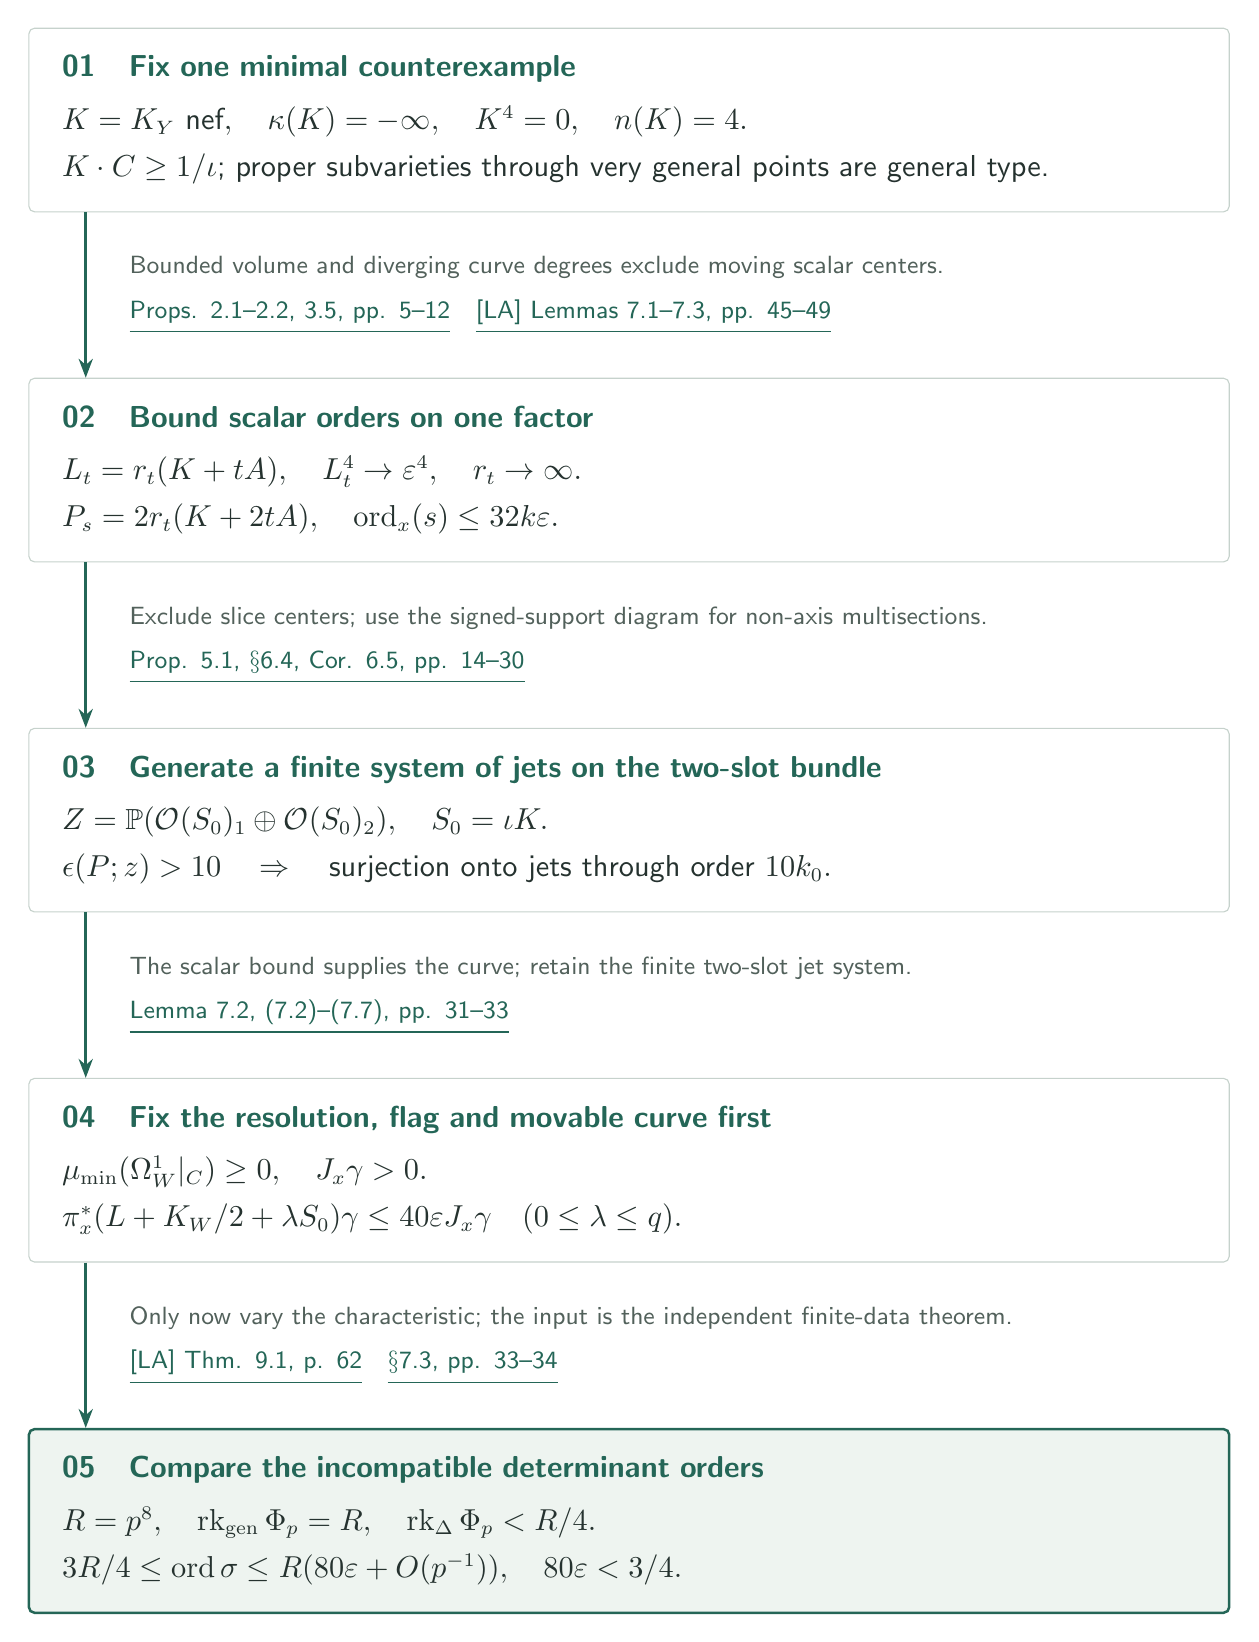
\begin{tikzpicture}
\node[card] (n0) {\heading{01}{反例を一つの極小モデルに固定する}{Fix one minimal counterexample}\Tx{$K=K_Y\text{ nef},\quad \kappa(K)=-\infty,\quad K^4=0,\quad n(K)=4.$\\[3pt]$K\cdot C\ge1/\iota$。非常に一般の点を通る真の部分多様体は general type。}{$K=K_Y\text{ nef},\quad \kappa(K)=-\infty,\quad K^4=0,\quad n(K)=4.$\\[3pt]$K\cdot C\ge1/\iota$; proper subvarieties through very general points are general type.}};
\node[card,below=2.1cm of n0] (n1) {\heading{02}{一因子上の消滅次数を小さく抑える}{Bound scalar orders on one factor}\Tx{$L_t=r_t(K+tA),\quad L_t^4\to\varepsilon^4,\quad r_t\to\infty.$\\[3pt]$P_s=2r_t(K+2tA),\quad\operatorname{ord}_x(s)\le32k\varepsilon.$}{$L_t=r_t(K+tA),\quad L_t^4\to\varepsilon^4,\quad r_t\to\infty.$\\[3pt]$P_s=2r_t(K+2tA),\quad\operatorname{ord}_x(s)\le32k\varepsilon.$}};
\flow{n0}{n1}{\Tx{体積は有界、曲線次数は発散。動く中心の次数上界から矛盾を得る。}{Bounded volume and diverging curve degrees exclude moving scalar centers.}\\[4pt]\Cite{fn}{Props. 2.1--2.2, 3.5, pp. 5--12}\quad \Cite{la}{[LA] Lemmas 7.1--7.3, pp. 45--49}}
\node[card,below=2.1cm of n1] (n2) {\heading{03}{二因子の束上で有限個のジェットを生成する}{Generate a finite system of jets on the two-slot bundle}\Tx{$Z=\mathbb P(\mathcal O(S_0)_1\oplus\mathcal O(S_0)_2),\quad S_0=\iota K.$\\[3pt]$\epsilon(P;z)>10\quad\Rightarrow\quad 10k_0\text{ 次ジェット全射。}$}{$Z=\mathbb P(\mathcal O(S_0)_1\oplus\mathcal O(S_0)_2),\quad S_0=\iota K.$\\[3pt]$\epsilon(P;z)>10\quad\Rightarrow\quad\text{surjection onto jets through order }10k_0.$}};
\flow{n1}{n2}{\Tx{sliceの中心を除く。非軸multisectionには符号付き台の図を使う。}{Exclude slice centers; use the signed-support diagram for non-axis multisections.}\\[4pt]\Cite{fn}{Prop. 5.1, $\S$6.4, Cor. 6.5, pp. 14--30}}
\node[card,below=2.1cm of n2] (n3) {\heading{04}{解消・旗・曲線を先に固定する}{Fix the resolution, flag and movable curve first}\Tx{$\mu_{\min}(\Omega_W^1|_C)\ge0,\quad J_x\gamma>0.$\\[3pt]$\pi_x^*(L+K_W/2+\lambda S_0)\gamma\le40\varepsilon J_x\gamma\quad(0\le\lambda\le q).$}{$\mu_{\min}(\Omega_W^1|_C)\ge0,\quad J_x\gamma>0.$\\[3pt]$\pi_x^*(L+K_W/2+\lambda S_0)\gamma\le40\varepsilon J_x\gamma\quad(0\le\lambda\le q).$}};
\flow{n2}{n3}{\Tx{scalar評価から曲線を選び、二因子ジェットと同時に有限データを固定する。}{The scalar bound supplies the curve; retain the finite two-slot jet system.}\\[4pt]\Cite{fn}{Lemma 7.2, (7.2)--(7.7), pp. 31--33}}
\node[result,below=2.1cm of n3] (n4) {\heading{05}{二つの行列式消滅次数を衝突させる}{Compare the incompatible determinant orders}\Tx{$R=p^8,\quad\operatorname{rk}_{\rm gen}\Phi_p=R,\quad\operatorname{rk}_{\Delta}\Phi_p<R/4.$\\[3pt]$3R/4\le\operatorname{ord}\sigma\le R(80\varepsilon+O(p^{-1})),\quad80\varepsilon<3/4.$}{$R=p^8,\quad\operatorname{rk}_{\rm gen}\Phi_p=R,\quad\operatorname{rk}_{\Delta}\Phi_p<R/4.$\\[3pt]$3R/4\le\operatorname{ord}\sigma\le R(80\varepsilon+O(p^{-1})),\quad80\varepsilon<3/4.$}};
\flow{n3}{n4}{\Tx{この段階で標数を動かす。入力は独立した有限データ定理である。}{Only now vary the characteristic; the input is the independent finite-data theorem.}\\[4pt]\Cite{la}{[LA] Thm. 9.1, p. 62}\quad \Cite{fn}{$\S$7.3, pp. 33--34}}
\end{tikzpicture}
\end{document}
